\PassOptionsToPackage{table}{xcolor}
\documentclass[12pt,letterpaper,twocolumn,openany,nodeprecatedcode,bg=none]{dndbook}
\usepackage[english]{babel}
\usepackage[utf8]{inputenc}
\usepackage{longtable,booktabs,array}
\usepackage{calc}
\usepackage{etoolbox}
\usepackage{caption}
\usepackage{float}
\usepackage{graphicx}
\usepackage{needspace}
\usepackage{tikz}

% Reset zebra striping at the start of every table
\AtBeginEnvironment{longtable}{\rowcolors{1}{white}{gray!10}\small}
\AtBeginEnvironment{table}{\rowcolors{1}{white}{gray!10}}

\providecommand{\pandocbounded}[1]{#1}
\providecommand{\tightlist}{%
  \setlength{\itemsep}{0pt}\setlength{\parskip}{0pt}}

\captionsetup{labelformat=empty}
\setcounter{secnumdepth}{0}
\setlength{\parindent}{0pt}
\setlength{\parskip}{0.5\baselineskip}
\setlength{\headheight}{15pt}

% Prevent orphaned subsections
\let\oldsubsection\subsection
\renewcommand{\subsection}[1]{%
  \needspace{5\baselineskip}%
  \oldsubsection{#1}%
}

\begin{document}
\onecolumn

      \title{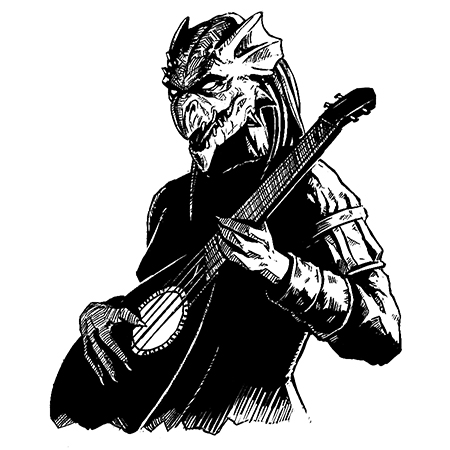
\includegraphics[width=0.9\textwidth,height=0.55\textheight,keepaspectratio]{bard.jpg}\\[1.5cm]Bard}
  \author{Class Handbook}
\date{}
\maketitle



\clearpage
\twocolumn

\section{Bard}\label{bard}

\subsection{Core Bard Traits}\label{core-bard-traits}

\needspace{13\baselineskip}

{\def\LTcaptype{none} % do not increment counter
\begin{table}[!htbp]
\centering
\begin{tabular}{@{}
  >{\raggedright\arraybackslash}p{(\linewidth - 2\tabcolsep) * \real{0.3377}}
  >{\raggedright\arraybackslash}p{(\linewidth - 2\tabcolsep) * \real{0.6623}}@{}}
\toprule\noalign{}
\begin{minipage}[b]{\linewidth}\raggedright
\textbf{Primary Ability}
\end{minipage} & \begin{minipage}[b]{\linewidth}\raggedright
Charisma
\end{minipage} \\
\midrule\noalign{}
\textbf{Hit Points} & 1d4 \\
\textbf{Saving Throw Proficiencies} & Dexterity, Charisma \\
\textbf{Skill Proficiencies} & Choose 4 skills \\
\textbf{Musical Proficiencies} & Choose 2 instruments \\
\textbf{Weapon Proficiencies} & Choose 2 categories \\
\textbf{Starting Equipment} & Padded Jacket, Dagger, Sabre, 2 Musical
Instruments \\
\bottomrule\noalign{}
\end{tabular}
\end{table}
}

\subsection{Bard Features}\label{bard-features}

\needspace{20\baselineskip}

{\def\LTcaptype{none} % do not increment counter
\begin{table}[!htbp]
\centering
\begin{tabular}{@{}
  >{\raggedright\arraybackslash}p{(\linewidth - 4\tabcolsep) * \real{0.0758}}
  >{\raggedright\arraybackslash}p{(\linewidth - 4\tabcolsep) * \real{0.1667}}
  >{\raggedright\arraybackslash}p{(\linewidth - 4\tabcolsep) * \real{0.7576}}@{}}
\toprule\noalign{}
\begin{minipage}[b]{\linewidth}\raggedright
Level
\end{minipage} & \begin{minipage}[b]{\linewidth}\raggedright
Proficiency
\end{minipage} & \begin{minipage}[b]{\linewidth}\raggedright
Class Features
\end{minipage} \\
\midrule\noalign{}
1 & +2 & Bardic Influence, Bardic Inspiration, Bardic Magic \\
2 & +2 & --- \\
3 & +2 & Ability Bonus \\
4 & +2 & --- \\
5 & +2 & --- \\
6 & +2 & --- \\
7 & +2 & Ability Bonus \\
8 & +2 & --- \\
9 & +3 & --- \\
10 & +3 & --- \\
\bottomrule\noalign{}
\end{tabular}
\end{table}
}

\subsection{Level 1: Bardic Influence}\label{level-1-bardic-influence}

People and creatures take a natural liking to you. When you roll
initiative, you can also make a DC 10 Charisma check. If you succeed,
you call a truce and give both sides the opportunity to interact. If
either side does something to offend the other, combat begins as normal.
Otherwise, you have the chance to negotiate a truce.

\subsection{Level 1: Bardic
Inspiration}\label{level-1-bardic-inspiration}

During combat, your singing and oration inspire others. On your turn,
you gain Bardic Inspiration dice based on your level. When you gain the
dice, you can keep them or give some or all of them to friendly
creatures that can hear you. A creature can roll a Bardic Inspiration
die and add the result as a bonus to an attack roll, a damage roll, or a
saving throw. Dice must be spent before rolling the d20 or damage.

All dice you gained on your last turn are lost at the start of your next
turn when you regain your dice.

\needspace{20\baselineskip}

{\def\LTcaptype{none} % do not increment counter
\begin{table}[!htbp]
\centering
\begin{tabular}{@{}
  >{\raggedright\arraybackslash}p{(\linewidth - 2\tabcolsep) * \real{0.1786}}
  >{\raggedright\arraybackslash}p{(\linewidth - 2\tabcolsep) * \real{0.8214}}@{}}
\toprule\noalign{}
\begin{minipage}[b]{\linewidth}\raggedright
Level
\end{minipage} & \begin{minipage}[b]{\linewidth}\raggedright
Bardic Inspiration Dice
\end{minipage} \\
\midrule\noalign{}
1 & 1d6 \\
2 & 1d6 \\
3 & 2d6 \\
4 & 2d6 \\
5 & 3d6 \\
6 & 3d6 \\
7 & 4d6 \\
8 & 4d6 \\
9 & 5d6 \\
10 & 5d6 \\
\bottomrule\noalign{}
\end{tabular}
\end{table}
}

\subsection{Level 1: Bardic Magic}\label{level-1-bardic-magic}

You pick up a strange mix of magic from your travels and studies. The
table below summarizes when you learn spells. When you gain a spell,
pick another class and roll on its table of your new spell's level. You
learn that spell. Alternatively, you can learn a spell taught to you by
a tutor, scroll, or other source of magic found during your adventure's
as determined by the DM. Charisma is your spellcasting ability for all
spells and magic abilities you learn.

After you cast the spell, you cannot cast it again until you finish a
long rest unless the spell is a cantrip. You cast a non-cantrip spell as
if you used a spell slot equal to the spell's level.

The `C' column is for cantrips.

\needspace{13\baselineskip}

{\def\LTcaptype{none} % do not increment counter
\begin{table}[!htbp]
\centering
\begin{tabular}{@{}
  >{\raggedright\arraybackslash}p{(\linewidth - 6\tabcolsep) * \real{0.3571}}
  >{\raggedright\arraybackslash}p{(\linewidth - 6\tabcolsep) * \real{0.2143}}
  >{\raggedright\arraybackslash}p{(\linewidth - 6\tabcolsep) * \real{0.2143}}
  >{\raggedright\arraybackslash}p{(\linewidth - 6\tabcolsep) * \real{0.2143}}@{}}
\toprule\noalign{}
\begin{minipage}[b]{\linewidth}\raggedright
Level
\end{minipage} & \begin{minipage}[b]{\linewidth}\raggedright
C
\end{minipage} & \begin{minipage}[b]{\linewidth}\raggedright
1
\end{minipage} & \begin{minipage}[b]{\linewidth}\raggedright
2
\end{minipage} \\
\midrule\noalign{}
1 & 1 & -- & -- \\
2 & 1 & 1 & -- \\
4 & 2 & 1 & -- \\
6 & 2 & 2 & -- \\
8 & 2 & 2 & 1 \\
10 & 2 & 2 & 2 \\
\bottomrule\noalign{}
\end{tabular}
\end{table}
}

\subsection{Level 3: Ability Bonus}\label{level-3-ability-bonus}

You gain a +1 bonus to two different abilities of your choice.

\subsection{Level 7: Ability Bonus}\label{level-7-ability-bonus}

You gain a +1 bonus to two different abilities of your choice.

\onecolumn

\clearpage
\thispagestyle{empty}
\begin{center}
\vspace*{\fill}
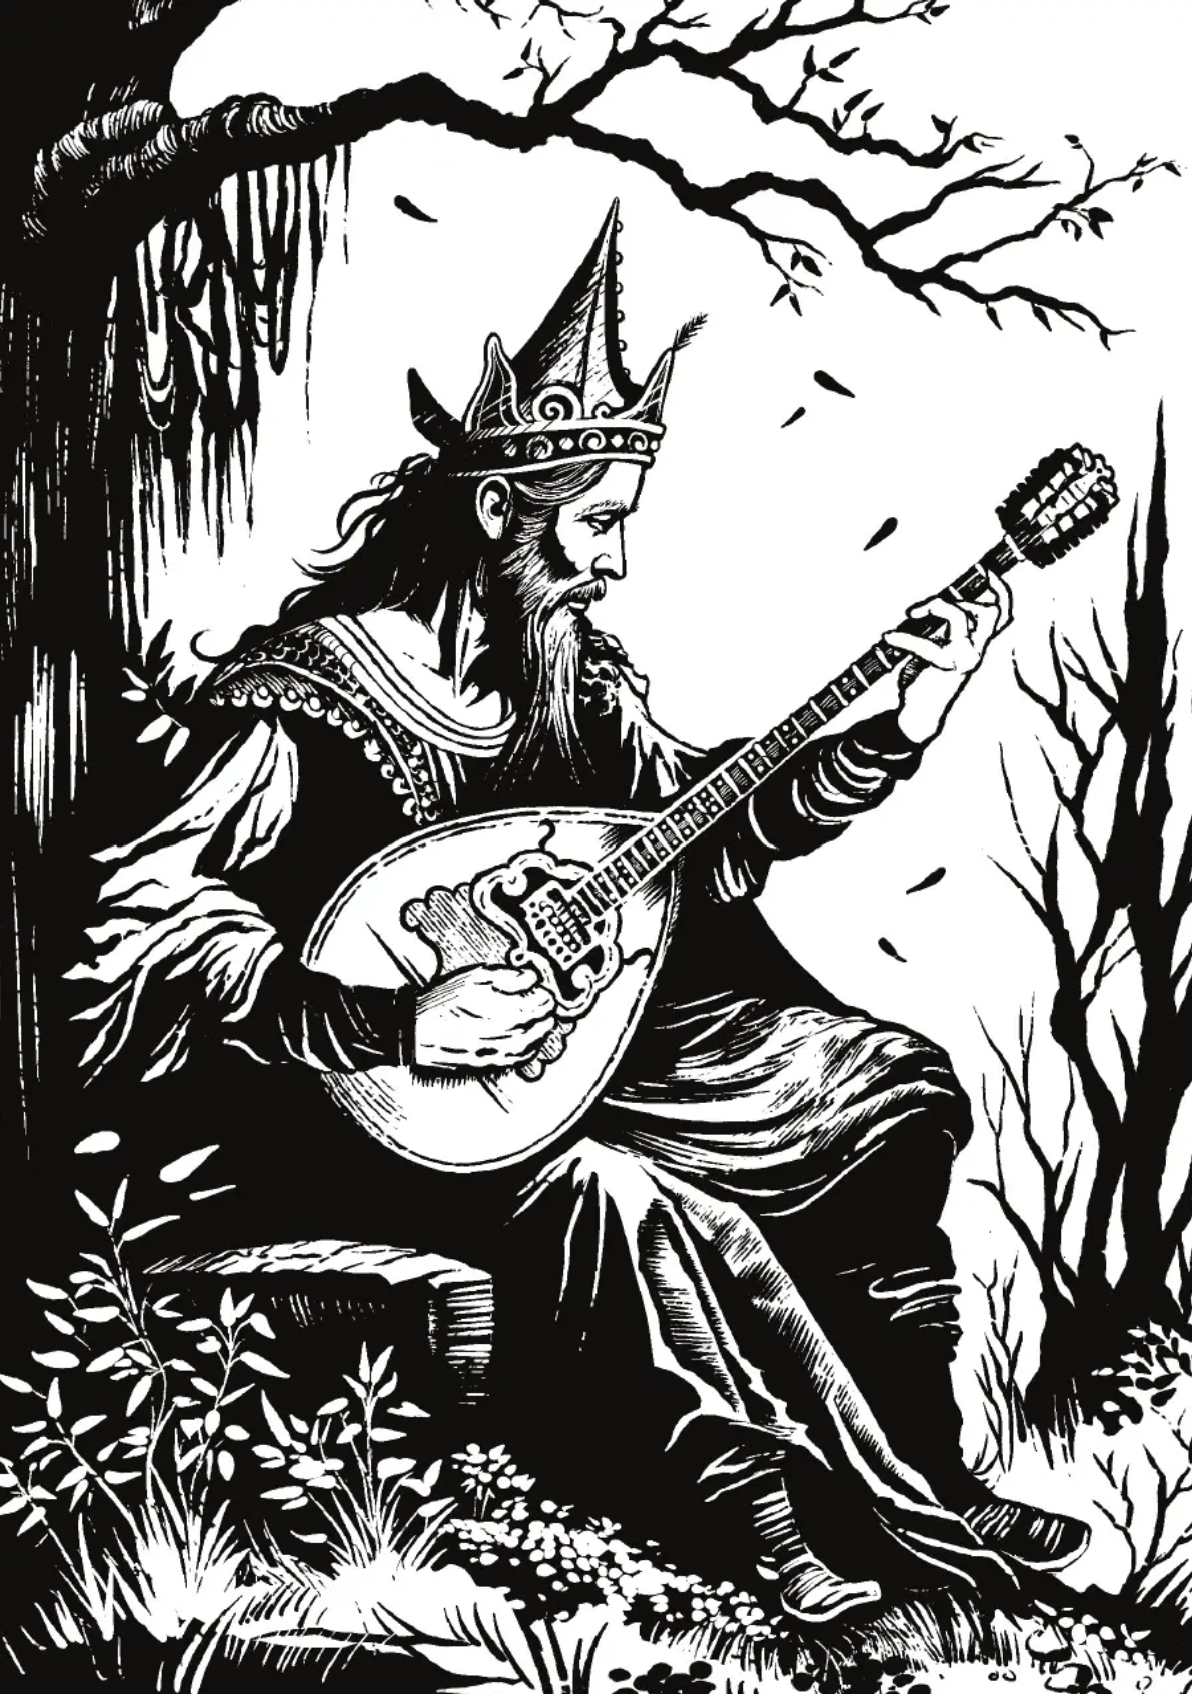
\includegraphics[width=0.7\textwidth,keepaspectratio]{bardSD.png}\par
\vspace{0.4cm}
{\itshape A bard is never alone so long as they have a song in their
heart.}\par
\vspace*{\fill}
\end{center}

\end{document}